\documentclass {article}
\usepackage{fullpage}
\usepackage{graphicx} % import images
\usepackage{listings}
\usepackage{url}
\usepackage{hyperref}
\usepackage{tikz}
\usepackage{wrapfig}
\usepackage{bchart}
\usetikzlibrary{shapes, arrows, calc, positioning}
\tikzstyle{line} = [draw, -latex']
\tikzstyle{block} = [rectangle, draw, text centered, rounded corners]
\tikzstyle{store} = [ellipse, draw, text centered]

\usepackage[parfill]{parskip}

\begin{document}

\begin{titlepage}
    \centering
    {\scshape\LARGE \phantom{.} \par}
    \vspace{2cm}
    {\scshape\LARGE University of Waterloo \par}
    \vspace{2cm}
    {\scshape\Large CS 488 Project Report\par}
    \vspace{2.5cm}
    {\huge\bfseries Generating Volumetric Terrain Procedurally Using the GPU\par}
    \vspace{2.5cm}
    {\LARGE\itshape Rudi Chen\par}
    {\Large r37chen\par}
    {\Large I.D. 20454807\par}

    \vfill

% Bottom of the page
    {\large \today\par}
\end{titlepage}

%----------------------------------------------------------------------------------------
%----------------------------------------------------------------------------------------
\section{Abstract}

This project is about generating high-quality volumetric terrain in OpenGL. We define a 3D terrain density function using Perlin Noise such that positive values represent the ground and negative values represent the air. The marching cubes algorithm is used to generate a mesh where the density value is zero. We use a variety of techniques to deal with texturing and lighting on a procedural mesh. Level-of-detail is implemented to render blocks farther away at lower resolutions allowing more blocks at once when navigating.

%----------------------------------------------------------------------------------------
%----------------------------------------------------------------------------------------
\section{Introduction}

The first procedural terrain generation techniques were significant innovations in computer graphics that allowed the creation of realistic landscapes. The classical technique is to create perturbations on a 2D grid using perlin noise or fractal algorithms. This is sometimes known as a 2.5D geometry.

\begin{center}
    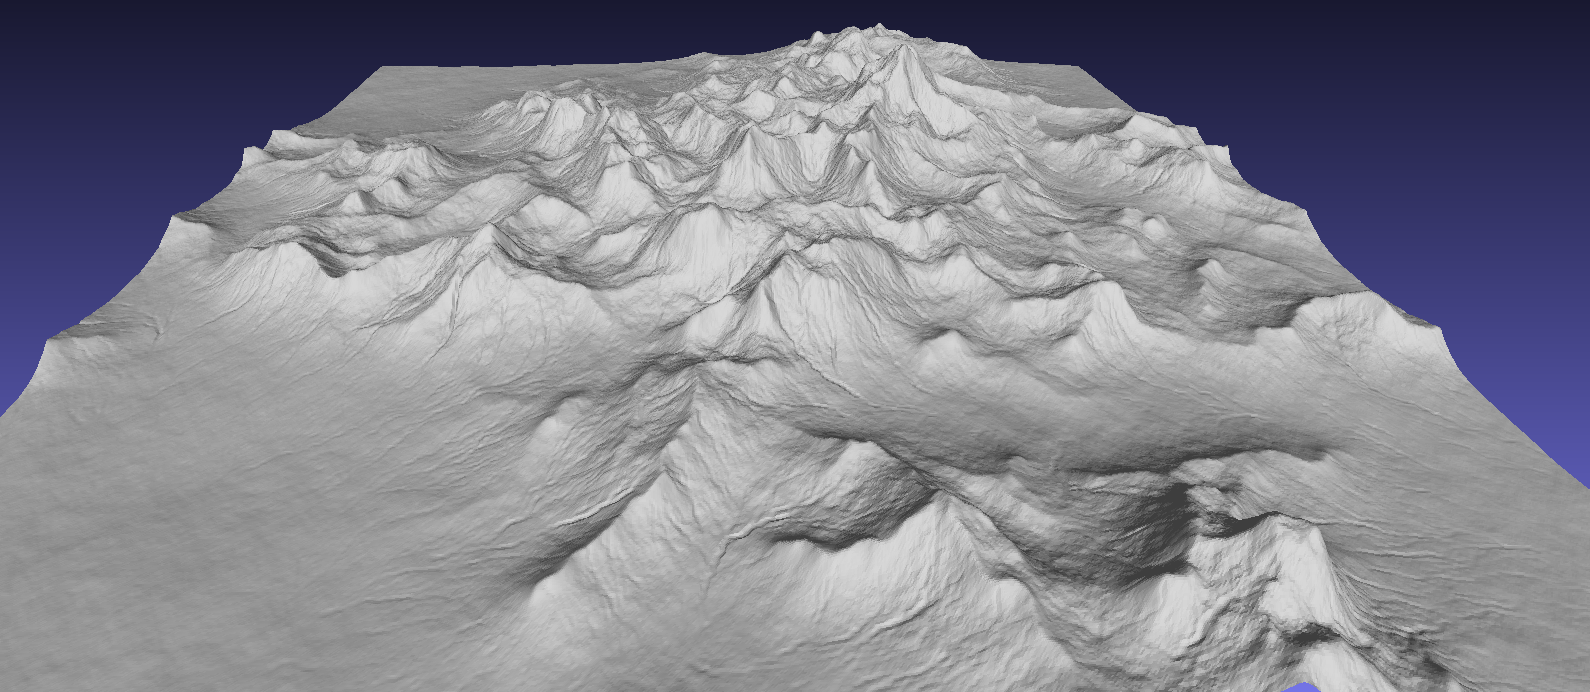
\includegraphics[width=12cm]{erosion.png}
\end{center}

While it is well suited for certain types of landscapes, such as mountains, this technique has limitations. As the geometry of the landscape is limited by a 2D mesh, it cannot support detailed features on vertical structures (e.g. protruding rock), overhangs or caves. This project uses a different technique to overcome those limitations by generating fully 3D complex terrain with features at all scales and angles in real-time using OpenGL.

The project is based on ``Generating Complex Procedural Terrain Using the GPU'' by Ryan Geiss, the first chapter from GPU Gems 3 \cite{Nguyen:2007:GG:1407436}. Here, terrain is generated as a density function in 32x32x32 voxel blocks using 3D Perlin noise, then converted to a mesh using the Marching Cubes algorithm, and rendered normally on the screen. For efficiency, this is implemented on the GPU - no data about the terrain ever needs to be transferred to or from the CPU. The stages of this process can be briefly summarized as such:

\vspace{5mm}

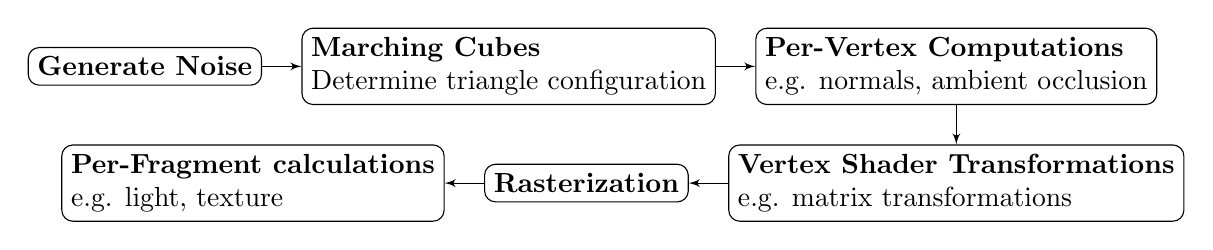
\begin{tikzpicture}[node distance=0.5cm, on grid=false]
\node [block] (noise) {\textbf{Generate Noise}};
\node [block, right=of noise, align=left] (marching) {\textbf{Marching Cubes} \\ Determine triangle configuration};
\node [block, right=of marching, align=left] (vertex) {\textbf{Per-Vertex Computations} \\ e.g. normals, ambient occlusion};
\node [block, below=of vertex, align=left] (vertex2) {\textbf{Vertex Shader Transformations} \\ e.g. matrix transformations};
\node [block, left=of vertex2, align=left] (raster) {\textbf{Rasterization}};
\node [block, left=of raster, align=left] (fragment) {\textbf{Per-Fragment calculations} \\ e.g. light, texture};
\path [line] (noise) -- (marching);
\path [line] (marching) -- (vertex);
\path [line] (vertex) -- (vertex2);
\path [line] (vertex2) -- (raster);
\path [line] (raster) -- (fragment);
\end{tikzpicture}

\vspace{5mm}

Although the CPU is mostly idle in the program, it is responsible for controlling the generation of blocks. Namely, level-of-detail is implemented to generate and render blocks further away at a lower resolution.

For more details, see the Implementations section.

% Needs to be here to be on this page...
\begin{wrapfigure}[30]{R}{0.25\linewidth}
    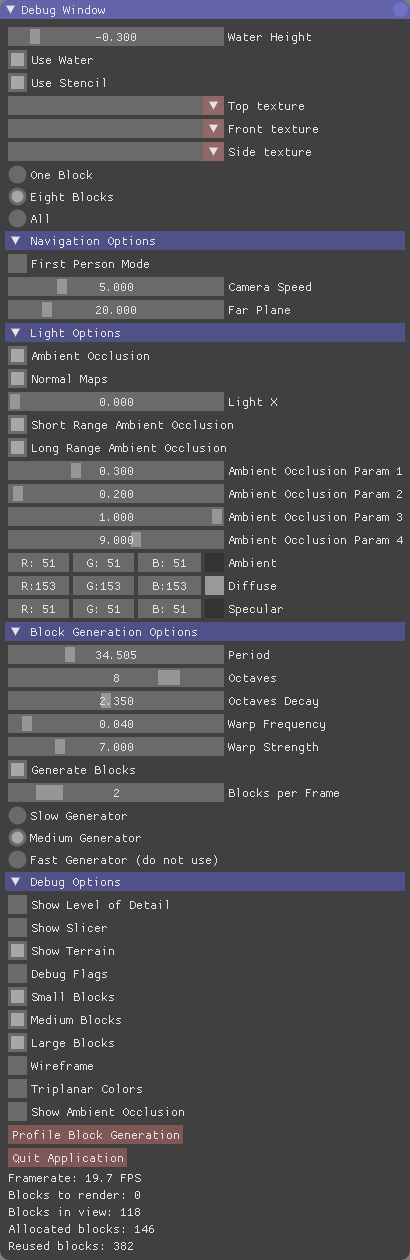
\includegraphics[width=6cm]{uipanel.png}
\end{wrapfigure}

%----------------------------------------------------------------------------------------
%----------------------------------------------------------------------------------------
\section{Manual}

The program can be compiled with the sequence of commands

\begin{lstlisting}
$ cd procedural-terrain-488
procedural-terrain-488$ premake4 gmake
procedural-terrain-488$ make
procedural-terrain-488$ cd src
procedural-terrain-488/src$ premake4 gmake
procedural-terrain-488/src$ make
\end{lstlisting}

And run with

\begin{lstlisting}
procedural-terrain-488/src$ ./procedural488
\end{lstlisting}

The program does not take any command-line arguments.

The program's UI panel contains options that can be toggled on and off. Most of them are just for debugging, but the ones of interest will be highlighted in bold below.

%----------------------------------------------------------------------------------------
\subsection{General Options}


\textit{Water Height}: Adjust the water level

\textit{Use Water}: Show water and reflection. Recommended to leave on.

\textit{Use Stencil}: Use a stencil so that the reflection of the terrain does not go past the boundaries in the water (only relevant when only 1 or 8 blocks are displayed.

\textit{Top Texture/Front Texture/Side Texture}: Choose the textures of the terrain (files are located in \texttt{src/Assets/Textures/}).

\textbf{One Block/Eight Blocks/All}: When this option is set to `All', every block within visible range will be drawn. However, changing terrain generation parameters often requires every block to be regenerated, which is too slow to be interactive. When playing with terrain parameters, it is recommended toggle to option to only render \textbf{Eight Blocks} at a time.

%----------------------------------------------------------------------------------------
\subsection{Navigation Options}

Initially, some terrain is generated and you can use the mouse to rotate the view about a fixed point, and the scrollwheel to zoom in and out.

First person navigation can be toggled with \textbf{First Person Mode}. In that mode, dragging with the mouse will rotate the camera in typical first-person style. The \textbf{WASD keys} allow you to move forward, backwards, and sideways. The \textbf{Q and E keys} move the camera up and down. You may want to increase the \textbf{Camera Speed}. The distance of the Far Plane can also be adjusted.

%----------------------------------------------------------------------------------------
\subsection{Light Options}

\textit{Ambient Occlusion}: Render parts of the terrain occluded by other parts of the terrain darker.

\textit{Normal Maps}: Use a normal map corresponding to the chosen textures.

\textit{Light X}: Move the light source in the x-axis, useful to visualize the interaction of the light with the terrain.

\textit{Short/Long Range Ambient Occlusion}: Whether to calculate ambient occlusion (regenerates all blocks).

\textit{Ambient Occlusion Params}: For debugging, affects the strength of ambient occlusion.

\textit{Ambient/Diffuse/Specular}: Color of the ambient, diffuse and specular components of the light source.

%----------------------------------------------------------------------------------------
\subsection{Block Generation Settings}

These settings should only be used when in \textbf{Eight Blocks} mode, as they require all blocks to be regenerated.

\textbf{Period}: This refers to the repetition period of the Perlin noise. In practice, this represents the distance between big terrain features.

\textbf{Octaves}: The number of samples of Perlin noise of different frequencies added together. A lower number means only large, smooth terrain features are rendered. A larger number means that the terrain is less smooth and contains smaller bumps.

\textit{Octaves decay}: The intensity of the smaller terrain features. A larger number means that the small variations in the terrain will be less visible.

Perlin noise is highly isotropic and looks too regular. To make the terrain richer and more varied, the noise samples are taken at a coordinate offset randomly by more Perlin noise.

\textit{Warp Frequency}: The frequency of the offset.

\textit{Warp Strength}: The strength of the offset.

\textit{Generate Blocks}: Check off to pause block generation.

\textit{Blocks per Frame}: Number of blocks to generate every frame. Increasing this number allows blocks to be generated faster, but may reduce the frame rate.

\textit{Slow/Medium Generator}: Switch between the two terrain generation methods (slow is 10x slower).

%----------------------------------------------------------------------------------------
\subsection{Debug Options}

\textbf{Show Level of Detail}: Draw colored transparent blocks to illustrate the size of the blocks being drawn on the screen at a particular frame. This visualization changes as the camera moves.

\textbf{Show Slicer}: Draw three planes to visualize 3D perlin noise. Use only in \textbf{Eight Blocks} mode.

\textit{Show Terrain}: Render the terrain.

\textit{Debug Flags}: Circumstantial, not currently used.

\textit{Small/Medium/Large Blocks}: Toggle on/off the rendering of blocks of size 1, 2 and 4 used in level of detail.

\textit{Wireframe}: Draw the terrain in wireframe mode.

\textit{Triplanar Color}: Show the direction of the normals and how they are used to blend together the 3 different textures.

\textit{Show Ambient Occlusion}: Draw the terrain in black and white, showing only the strength of ambient occlusion in different parts.

\textit{Profile Block Generation}: Render 100 blocks immediately and print the amount of time taken to the console.

%----------------------------------------------------------------------------------------
%----------------------------------------------------------------------------------------
\section{Code Documentation}


The general layout of the codebase is similar to the one provided in the previous the assignments. At the root level, we have folders \texttt{shared/} and \texttt{src/} . All libraries and code which we did not write is located in \texttt{shared/}. My project code and additional assets are located in \texttt{src/}.

%----------------------------------------------------------------------------------------
\subsection{Libraries}

In addition to the libraries used in previous CS 488 assignments (framework code, glfw, imgui), I use two libraries.

\begin{itemize}
\item OpenAL: This library provides a way to play sound in C++. It is quite powerful in that it has 3D sound features, such as adjusting the volume of a sound effect by distance. However, I only use it to play background music.
\item SOIL: This is a simple lightweight library which I used to read JPEG images.
\end{itemize}

The CS 488 framework was slightly modified so that \texttt{ShaderProgram} could load Compute Shaders and support inheritance, where the inherited object is \texttt{TransformProgram}, a specialized \texttt{ShaderProgram} that supports Transform Feedback (an OpenGL technique to write vertices to an array and skip rasterization).

%----------------------------------------------------------------------------------------
\subsection{Engine Code}

The main C++ codebase for the project are all contained in the \texttt{src/} folder. The two main files of interest are \texttt{navigation.cpp} and \texttt{block\_manager.cpp}: they contain most of the main logic and drive the code.

\subsubsection{Game Logic}

The class \texttt{Navigation} in \texttt{navigation.cpp} contains the code to create the UI, handle inputs, change parameters in the program, manage camera parameters, manage navigation at every frame, and call other parts of the code to draw the scene.

\subsubsection{Block Generation Logic}

All blocks are uniquely identified with a 4-component integer vector (\texttt{ivec4}). The first 3 components represent the location of the unit grid in 3D and the 4th component represents the size of the block (can be either 1, 2 or 4), which is used for level-of-detail rendering.

The class \texttt{BlockManager} in \texttt{block\_manager.cpp} stores a number of program parameters (e.g. whether to use ambient occlusion), the list of blocks currently visible in the scene and a memory pool of free block that contains OpenGL buffers representing allocated blocks of memory on the GPU. It also handles the logic of determining the best blocks to generate every frame, managing the block memory pool, creating new blocks, and rendering the scene. Rendering the scene includes drawing the blocks in the right order (since some might be transparent) and handling reflection.

The class \texttt{Block} in \texttt{block.cpp} contains the OpenGL objects storing the vertices that were generated for that block, a boolean to indicate whether the block has been generated, and its current transparency (for a smooth fade-in) which is updated every frame.

The class \texttt{TerrainRenderer} in \texttt{terrain\_renderer.cpp} stores the block rendering shader and the location of all uniforms and attributes needed to render the block, including textures.

The base class \texttt{TerrainGenerator} and its subclasses \texttt{TerrainGeneratorSlow} and \texttt{TerrainGeneratorMedium} handle the logic to generate the blocks (density volume and vertices).  This includes making the shader calls and piping the outputs to one another. The two variants are interchangeable and store the final output in the \texttt{Block} argument passed to \texttt{generateTerrainBlock(...)}.

The class \texttt{Lod} in \texttt{lod.cpp} stands for Level-Of-Detail and contains logic for determining which blocks are visible and need to be rendered or generated. Note that the function \texttt{generateForPosition(...)} takes in the current projection, view and world matrices, as well as the current eye position.

\subsubsection{Geometry}

Although most of the scene is a procedurally generated mesh, there is some geometry that follows the following class layout:

\vspace{5mm}

\begin{center}
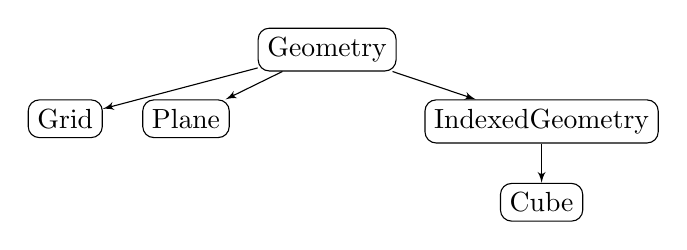
\begin{tikzpicture}[node distance=0.5cm, on grid=false]
\node [block] (geometry) {Geometry};
\node [block, below left=of geometry] (plane) {Plane};
\node [block, left=of plane] (grid) {Grid};
\node [block, below right=of geometry] (indexed) {IndexedGeometry};
\node [block, below=of indexed] (cube) {Cube};
\path [line] (geometry) -- (plane);
\path [line] (geometry) -- (grid);
\path [line] (geometry) -- (indexed);
\path [line] (indexed) -- (cube);
\end{tikzpicture}
\end{center}

\vspace{5mm}

This structure factors out some of the code to create Vertex Buffer Objects and Vertex Array Objects. An IndexedGeometry renders using vertex indices (\texttt{glDrawElements} instead of \texttt{glDrawArrays}).

\subsubsection{Debugging}

Some classes are used to visualize certain aspects of the program logic for debugging purposes. The class \texttt{DensitySlicer} in \texttt{density\_slicer.cpp} contains three planes and a shader to visualize slices of 3D perlin noise. The class \texttt{LodVisualizer} in \texttt{lod\_visualizer.cpp} is used to draw transparent cubes of different sizes and colors to visualize the blocks that need to be visible in the current scene from level-of-detail.

\subsubsection{Other}

There are various utility files, such as \texttt{constants.hpp} which holds program-wide constants like the resolution of a block, and \texttt{vec\_hash.hpp} which implements a hash function for glm integer vectors.

The classes \texttt{Texture}  and \texttt{Sound} in \texttt{texture.hpp} and \texttt{sound.hpp} store external texture and sound assets loaded in the program.

The class \texttt{Water} in \texttt{water.hpp} handles drawing the water.

Any other files not mentioned present in the source directory are work-in-progress files that were not used in the final demo.

%----------------------------------------------------------------------------------------
\subsection{Shaders}

GLSL code executed on the GPU is located in \texttt{src/Assets}. First, note that GLSL's modularity capabilities are non-existent. It is not even possible to include code for reuse. However, many methods are needed across multiple files, namely those related to marching cubes, in multiple files. The script \texttt{include.py} is run by the program at execution and replaces instances of \verb|#include "file.h"| with the textual content of the file and puts the output shader files in \texttt{src/Assets/out}. However, it is not recursive.

The reusable file \texttt{noise.h} contains functions to generate the 3D density function, \texttt{marching\_cubes\_common.h} contains all the lookup tables needed for marching cubes, and \texttt{terrain\_vertex\_common.h} has logic for vertex normals and ambient occlusion.

The rest of the shader files are organized in several pipelines as shown in the diagram below:

\vspace{5mm}

\begin{center}
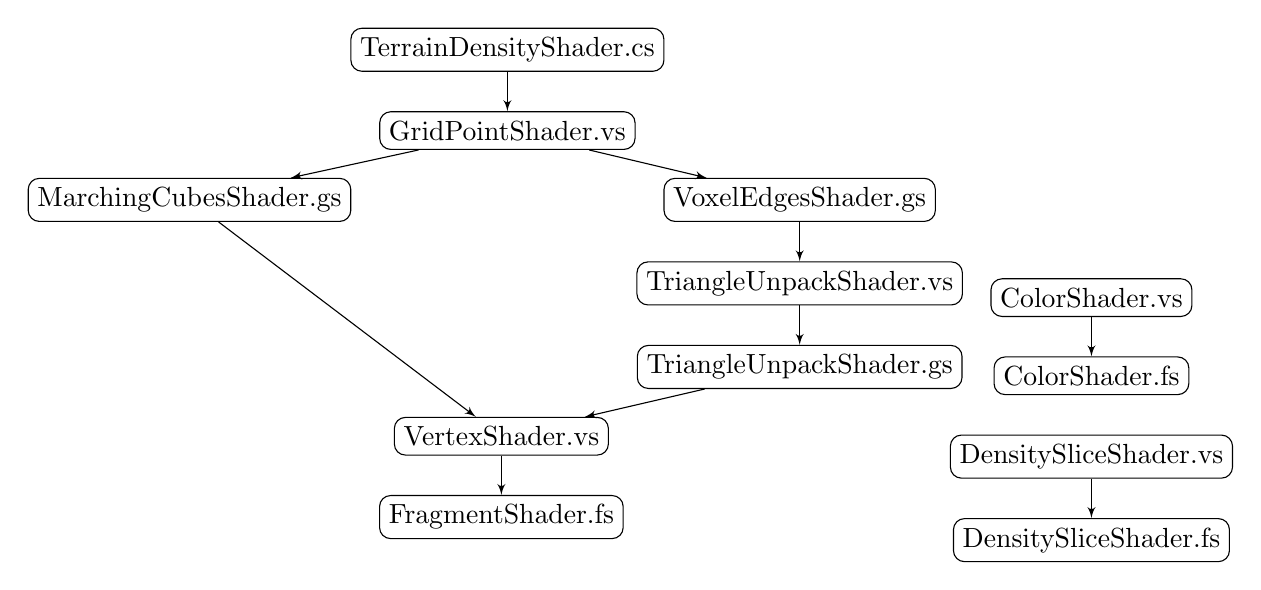
\begin{tikzpicture}[node distance=0.5cm, on grid=false]
\node [block] (terraindensity) {TerrainDensityShader.cs};
\node [block, below=of terraindensity] (gridpoint) {GridPointShader.vs};
\node [block, below left=of gridpoint] (marchingcubes) {MarchingCubesShader.gs};
\node [block, below right=of gridpoint] (voxeledges) {VoxelEdgesShader.gs};
\node [block, below=of voxeledges] (trianglevs) {TriangleUnpackShader.vs};
\node [block, below=of trianglevs] (trianglegs) {TriangleUnpackShader.gs};
\node [block, below left=of trianglegs] (vertex) {VertexShader.vs};
\node [block, below=of vertex] (fragment) {FragmentShader.fs};
\node [block, above right=of trianglegs] (colorvs) {ColorShader.vs};
\node [block, below=of colorvs] (colorfs) {ColorShader.fs};
\node [block, below=of colorfs] (densityslicevs) {DensitySliceShader.vs};
\node [block, below=of densityslicevs] (densityslicefs) {DensitySliceShader.fs};
\path [line] (terraindensity) -- (gridpoint);
\path [line] (gridpoint) -- (marchingcubes);
\path [line] (gridpoint) -- (voxeledges);
\path [line] (voxeledges) -- (trianglevs);
\path [line] (trianglevs) -- (trianglegs);
\path [line] (marchingcubes) -- (vertex);
\path [line] (trianglegs) -- (vertex);
\path [line] (vertex) -- (fragment);
\path [line] (colorvs) -- (colorfs);
\path [line] (densityslicevs) -- (densityslicefs);
\end{tikzpicture}
\end{center}

%----------------------------------------------------------------------------------------
%----------------------------------------------------------------------------------------
\section{Objectives}
\begin{enumerate}
 \item[\_\_\_ 1:]    Implement 3D Perlin Noise to generate a terrain density function.

 \item[\_\_\_ 2:]   Implement the Marching Cubes algorithm to generate triangles out of the density function.

 \item[\_\_\_ 3:]   Implement ambient occlusion by casting out shadow rays for each vertex.

 \item[\_\_\_ 4:]   Map textures onto the generated mesh by using triplanar texturing.

 \item[\_\_\_ 5:]   Implement bump mapping by mapping a bump map texture onto the generated mesh to perturb normal vectors.

 \item[\_\_\_ 6:]   Optimize terrain generation code by splitting terrain generation work into smaller units with multiple shader passes to eliminate redundant work (e.g. shared vertices) as described in the book chapter.

 \item[\_\_\_ 7:]   Implement level-of detail rendering and alpha blending to improve the transition between blocks of terrain of different resolutions from level-of-detail rendering, which will require rendering the blocks furthest away first.

 \item[\_\_\_ 8:]   UI: Create a first-person camera and appropriate controls to navigate the scene, including moving in all 3 axes, adjusting the movement speed and rotating the camera.

 \item[\_\_\_ 9:]   Modelling: Add geometry to represent water to the scene.

 \item[\_\_\_ 10:]  Implement reflection for water by rendering the scene onto a texture.
\end{enumerate}

%----------------------------------------------------------------------------------------
%----------------------------------------------------------------------------------------
\section{Implementation}

%----------------------------------------------------------------------------------------
\subsection{Terrain Density}

The terrain is defined by a 3D density function where positive values are the ground, negative values are the air, and the mesh is located where the function evaluates to zero. A key component of this function is 3D Perlin Noise.

Conceptually, Perlin Noise consists of random vectors at integer grid points representing the gradient of the function at that point, and the value of the function at any point is obtained by interpolating with an easing function. However, variations were introduced over the years when it comes to implementation details. In particular, we use two key variations described in \cite{Fernando:2004:GGP:983868}. First, the easing function used is $f(t) = 6t^5 - 15t^4 + 10t^3$, which has better continuity properties at its derivatives. Second, the random vectors is selected from a set of 12 vectors which point to the edges of a unit cube. The random vector generator can then simply select the vector based on the hash of the grid point. This is faster than generating fully random vectors and has the advantage that adjacent vectors are unlikely to be too similar, which tends to produce less pleasing results visually.

The sampling of the noise is `warped'. It is distorted (the coordinate is offset) by another sampling of two octaves of the Perlin noise, to reduce isotropy. In the code:

\begin{lstlisting}
vec3 warped_coords = coords;
warped_coords += perlinNoise(coords, warp_params.x) * warp_params.y;
warped_coords += perlinNoise(coords, warp_params.x * 1.9) * (warp_params.y / 2);
\end{lstlisting}

A few samples of Perlin noise at different frequencies are added together to get details at all scales.

\begin{lstlisting}
float noise = 0.0;
float frequency = 1.0 / period;
for (int i = 1; i <= octaves; i++) {
    noise += perlinNoise(warped_coords, frequency) / pow(i, octaves_decay);
    frequency *= 1.95;
}
\end{lstlisting}

A gradient from 0 to 1.5 is then added to the noise in the y-direction, in order to force the transition from ground to air.

%----------------------------------------------------------------------------------------
\subsection{Marching Cubes}

The implementation of Marching Cubes is fairly standard\cite{Lorensen:1987:MCH:37401.37422}. For every voxel, the density value at the 8 corners of the cube determine which of 256 triangle configurations is used for that voxel. Each configuration can have up to 5 triangles, each of which is stored as an integer representing one of the 12 edges on the cube. The exact location of the vertex on that edge is proportional to the density value at the two ends of the edge.

\begin{center}
    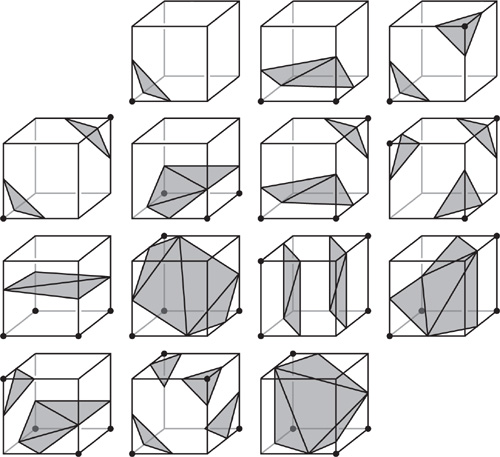
\includegraphics[width=5cm]{marchingcubes.jpg}
\end{center}

The difficulty lies in implementing this technique in the various shader stages of the GPU. In particular, we demonstrate two techniques, one which is significantly faster than the other.

\vspace{5mm}
\begin{center}
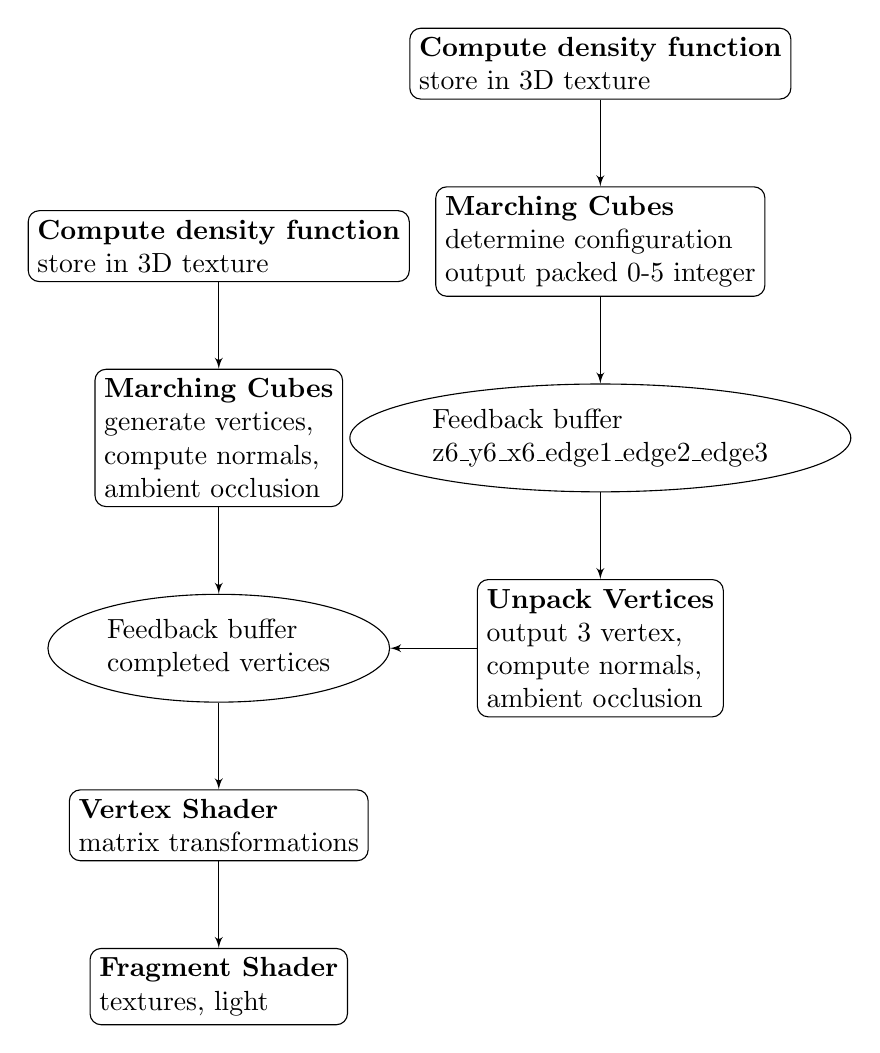
\begin{tikzpicture}[node distance=1.1cm]
\node [block, align=left] (density) {\textbf{Compute density function} \\ store in 3D texture};
\node [block, below=of density, align=left] (marching) {\textbf{Marching Cubes} \\ generate vertices, \\ compute normals, \\ ambient occlusion};
\node [store, below=of marching, align=left] (marchingfeedback) {Feedback buffer\\completed vertices};
\node [block, below=of marchingfeedback, align=left] (vertex) {\textbf{Vertex Shader} \\ matrix transformations};
\node [block, below=of vertex, align=left] (fragment) {\textbf{Fragment Shader} \\ textures, light};
\node [block, right=of marchingfeedback, align=left] (unpack) {\textbf{Unpack Vertices} \\ output 3 vertex, \\ compute normals, \\ ambient occlusion};
\node [store, above=of unpack, align=left] (packedfeedback) {Feedback buffer\\z6\_y6\_x6\_edge1\_edge2\_edge3};
\node [block, above=of packedfeedback, align=left] (case) {\textbf{Marching Cubes} \\ determine configuration \\ output packed 0-5 integer};
\node [block, above=of case, align=left] (grid) {\textbf{Compute density function} \\ store in 3D texture};
\path [line] (density) -- (marching);
\path [line] (marching) -- (marchingfeedback);
\path [line] (marchingfeedback) -- (vertex);
\path [line] (vertex) -- (fragment);
\path [line] (grid) -- (case);
\path [line] (case) -- (packedfeedback);
\path [line] (packedfeedback) -- (unpack);
\path [line] (unpack) -- (marchingfeedback);
\end{tikzpicture}
\end{center}

\vspace{5mm}

First, in both cases, the first step is to generate a 32x32x32 3D texture representing the terrain density. Then, marching cubes is applied in order to convert density values into a triangle mesh. To do so, it is necessary to be able to generate vertices inside the GPU. The key technology that enables this is the Geometry Shader, which takes in a vertex and outputs an arbitrary number of vertices. In this case, the input vertex comes from a 31x31 grid instanced 31 times, such that each vertex represents a voxel. Note that a NxNxN voxel grid needs (N+1)x(N+1)x(N+1) samples of the texture.

In the slow implementation (left), the Geometry Shader is used only once. It is responsible for reading the density value, determining the Marching Cubes triangle configuration, and calculating vertex position, normals and ambient occlusion. In the code, this looks like

\begin{lstlisting}
int case_index = ... // marching cube configuration (0-255)
int numpolys = case_to_numpolys[case_index]; // number of polygons in this configuration
for (int i = 0; i < numpolys; i++) {
    ...
    vec3 v1 = ... // position of vertex 1
    vec3 v2 = ... // position of vertex 2
    vec3 v3 = ... // position of vertex 3

    createVertex(v1); // calculate normal and ambient occlusion for v1
    EmitVertex();
    createVertex(v2); // calculate normal and ambient occlusion for v1
    EmitVertex();
    createVertex(v3); // calculate normal and ambient occlusion for v1
    EmitVertex();

    EmitPrimitive(); // one triangle
}
\end{lstlisting}

Note that for every voxel, the Geometry Shader will output 0 to 15 vertices, since each marching cube configuration can have up to 5 triangles. Each vertex consistent of 7 floats (position, normal and ambient occlusion).

Why is this slow? The GPU follows the SIMD (Single Instruction Multiple Data) model of computation. Typically, the input data is partitioned into groups. Different GPU programming libraries use different terminologies for such a group (work group, thread block, etc). In each group, each input datum (here, the position of a voxel) is processed by one thread assigned to one core, and a few thousand cores execute simultaneously with the same set of instructions.

Due to the presence of branching in the Geometry Shader, not all threads within a group will finish at the same time. However, all threads must finish before the next thread group begins. As such, many cores in the GPU will sit idle. If any thread in the group needs to generate 15 vertices, then all threads in the group will be idle until the number of cycles needed to generate 15 vertices.

The faster approach (right) solves this problem by minimizing thread idle time. Here, the first Geometry Shader determines the Marching Cubes configuration for each voxel. Then, each triangle in the configuration is output as an integer which uses bit packing to store the coordinate of the voxel and the indices of the edges of a cube corresponding to the vertices of the triangle. As such, the first Geometry Shader outputs 0 to 5 integers. While there is still some idle time, it is minimized, since none of this idle time is spent waiting on expensive floating-point operations and array lookups to calculate the vertex positions and ambient occlusion.

The second Geometry Shader takes this packed integer and calculates the vertex positions and ambient occlusion. However, since every packed integer corresponds to one triangle, every thread will output exactly 3 vertices, so there is no idle time. The graph below shows the time taken to generate 100 32x32x32 blocks in seconds using the fast and slow techniques.

\begin{center}
\begin{bchart}[step=2,max=10]
    \bcbar[label=Fast (no AO)]{0.56}
        \smallskip
    \bcbar[label=Fast (AO)]{0.69}
        \smallskip
    \bcbar[label=Slow (no AO)]{1.24}
        \smallskip
    \bcbar[label=Slow (AO)]{9.28}
\end{bchart}
\end{center}

The graph also shows the timing results when long-range ambient occlusion is disabled, the most expensive per-vertex calculation. Note that the speedup is much greater using the slow pipeline when long-range ambient occlusion is disabled, demonstrating that many cores sit idle when other cores are busy computing long-range ambient occlusion.

%----------------------------------------------------------------------------------------
\subsection{Ambient Occlusion}

Ambient Occlusion is a type of shadowing technique that approximates the amount of light that can reach any given area on a mesh, independently of light position. One common way to calculate this is by sending light rays in random directions and checking if they hit anything. Generally, light rays sent from points in concave areas will hit more geometry and hence, be considered to be located in a darker area.

Normally, this type of ambient occlusion is too expensive to be used in real-time applications since intersecting light rays with triangles in the GPU is difficult. However, in this case, we can use the density function instead of triangle geometry to determine the presence of terrain.

Our ambient occlusion has two components: short-range and long-range.

Short-range ambient occlusion sends rays up to a distance of 4 units away and samples the texture to get the density value. Note that this requires us to generate a larger texture to deal with sampling beyond the edges, but generating the density function is not a bottleneck to begin with, so the cost is not significantly increased.

Long-range ambient occlusion sends rays up to a distance of 30 units away. In this case, it would not be practical to generate a texture large enough. Instead, the density value is computed from the density function directly. Since this is expensive, the density value along long-range rays is only sampled 5 times.

\begin{center}
    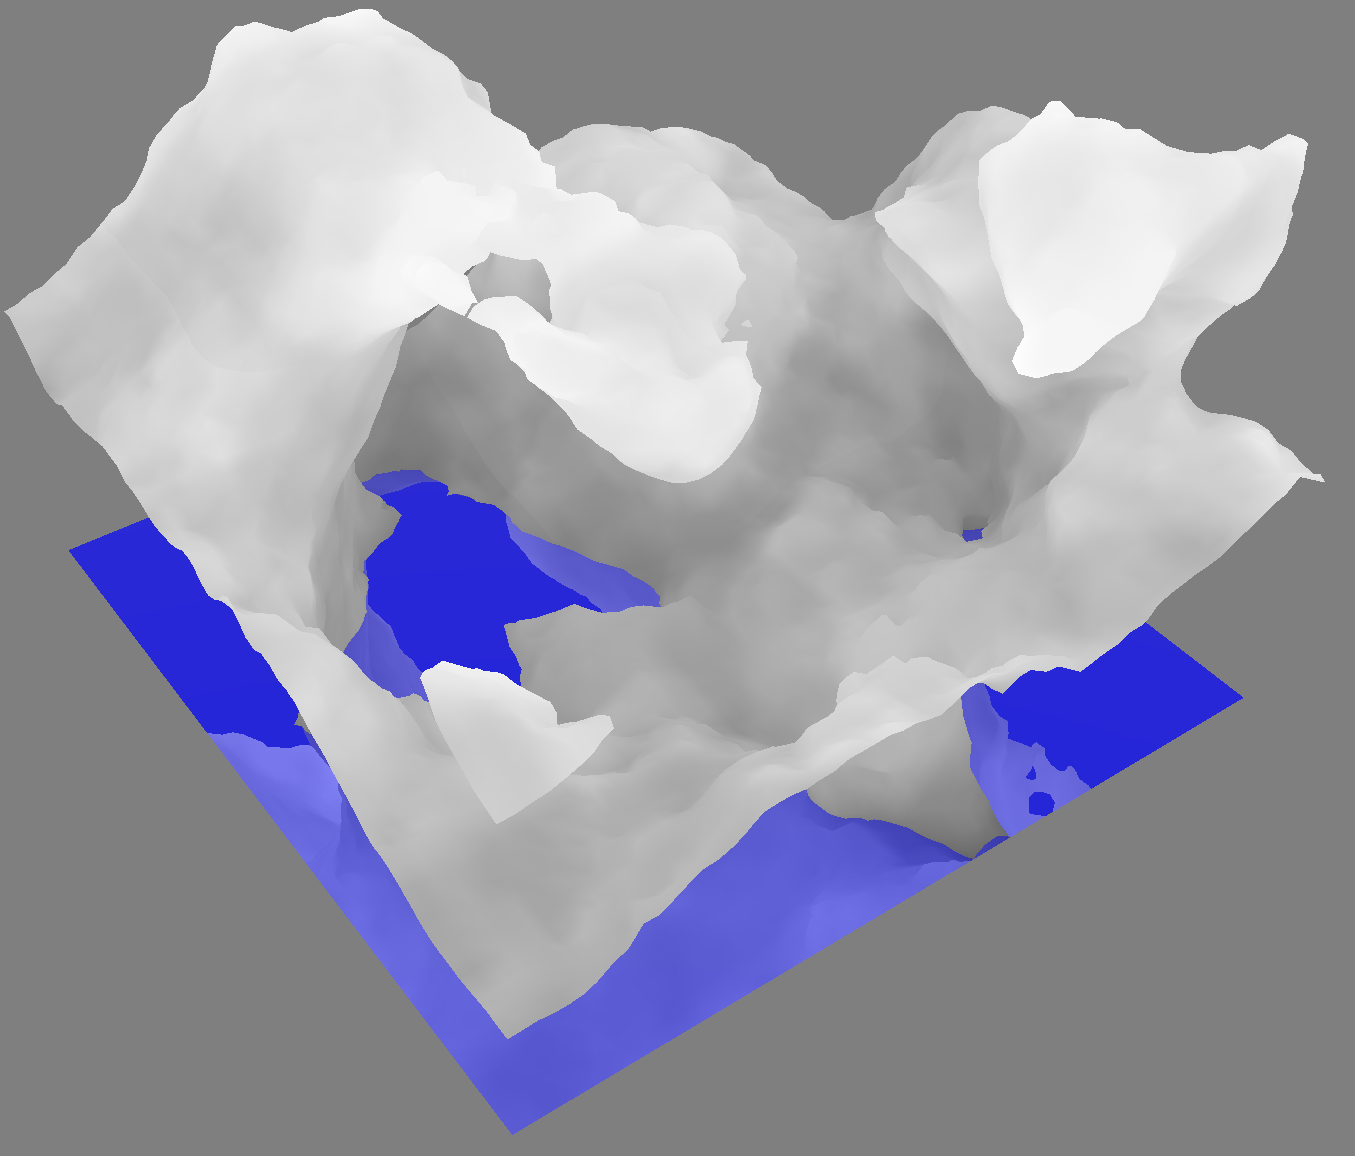
\includegraphics[width=6cm]{ambientocclusion.png}

    ambient occlusion visualization
\end{center}

%----------------------------------------------------------------------------------------
\subsection{Texturing}

Applying a texture on an arbitrary procedurally generated mesh is challenging. If not careful, the texture can be stretched when the angle is too steep, as shown below.

\begin{center}
    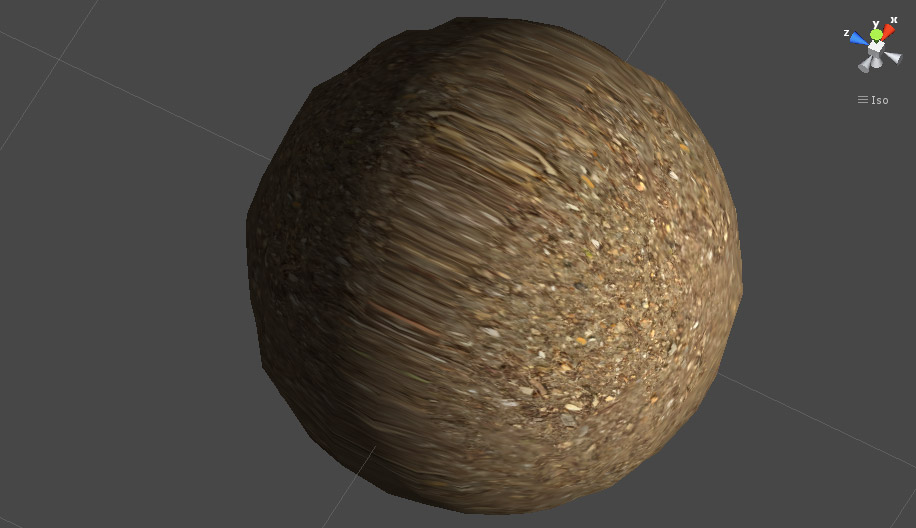
\includegraphics[width=6cm]{planetoid.jpg}

    \textit{Image from http://answers.unity3d.com/questions/422086/applying-texture-to-quads-on-procedural-cube.html}
\end{center}

To resolve this issue, instead of applying one texture, we apply three textures: one in the direction of the x-axis ($(u,v) = (-v.z, -v.y)$), one in the direction of the y-axis ($(u, v) = (v.x, v.z)$), and one in the direction of the z-axis ($(u, v) = (v.x, -v.y)$). This is a technique called \textbf{triplanar texturing}. To select which texture to use at any given pixel, we use the value of the normal vector. The image below illustrates the weight assigned to each texture, represented in three different shades of gray. Note that the weights transitions smoothly from one to another. These calculations can all be done in the Fragment Shader.

\begin{center}
    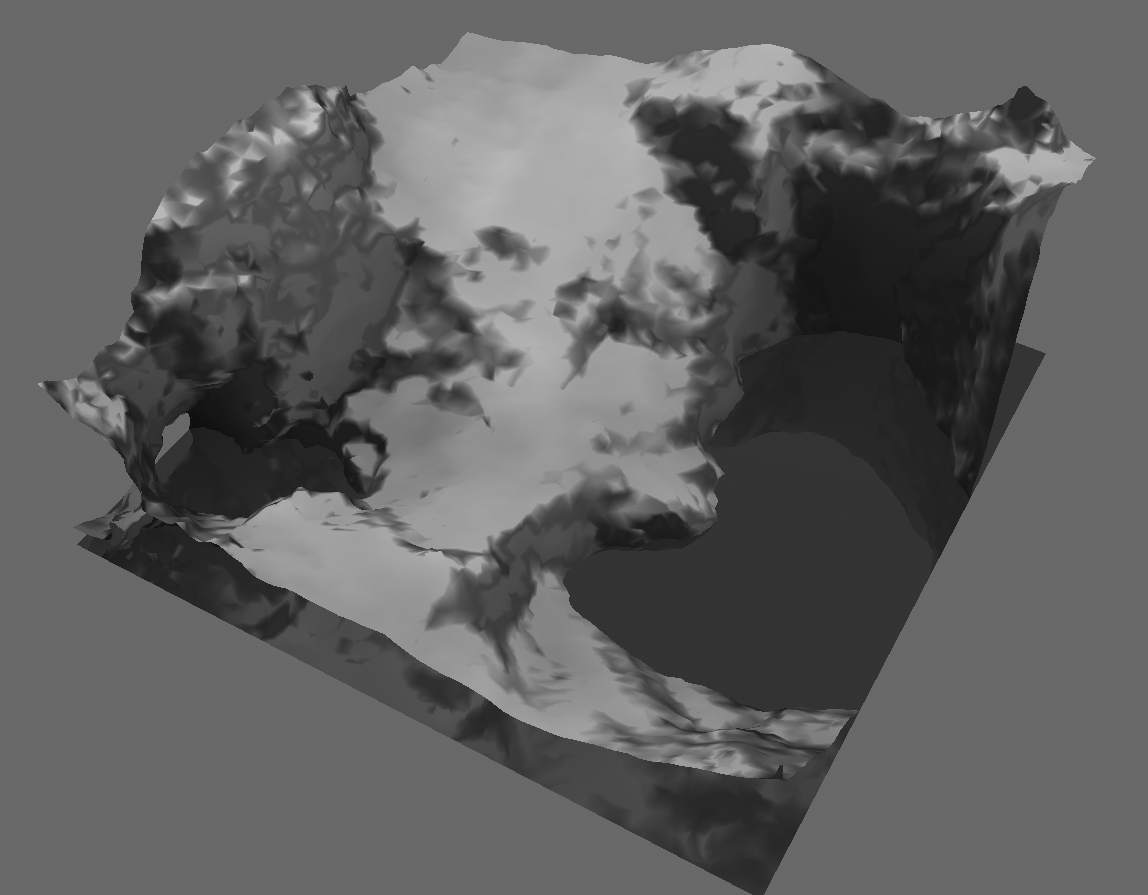
\includegraphics[width=7cm]{triplanar.png}

    triplanar texturing weights visualization
\end{center}

The normal vector is calculated by simply taking the gradient of the density function as shown below.

\begin{lstlisting}
vec3 normalAtVertex(vec3 vertex)
{
    float d = 1.0; \\ epsilon (here, quite large)
    vec3 gradient = vec3(
        density(vertex + vec3(d, 0, 0)) - density(vertex - vec3(d, 0, 0)),
        density(vertex + vec3(0, d, 0)) - density(vertex - vec3(0, d, 0)),
        density(vertex + vec3(0, 0, d)) - density(vertex - vec3(0, 0, d)));
    return -normalize(gradient);
}
\end{lstlisting}

%----------------------------------------------------------------------------------------
\subsection{Bump Mapping}

We implement bump mapping by using one normal map for each of the three textures in triplanar texturing. A key difference between normal maps and regular textures is that it is necessary to know the orientation of the texture on each triangle, in addition to the UV coordinate.

In a normal map, the normal vectors are represented in tangent space, defined by a normal vector (N), tangent vector (T) and bi-tangent vector (B). In tangent space, normals generally point in the positive Z direction, stored in the blue component of the image, which is why normal maps always have a blue tint.

\begin{center}
    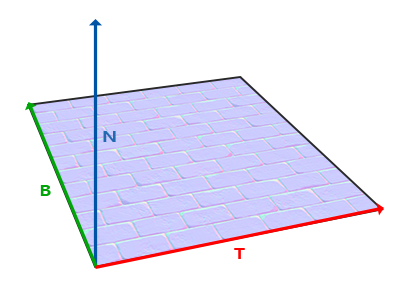
\includegraphics[width=6cm]{tbn1.png}
    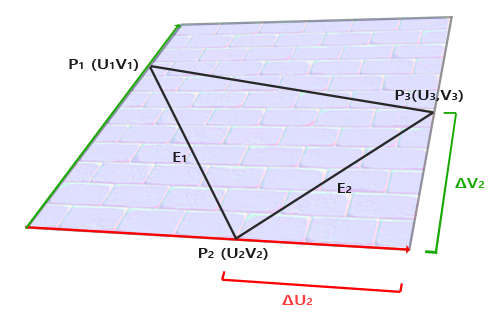
\includegraphics[width=6cm]{tbn2.png}

    \textit{Images from http://learnopengl.com/\#!Advanced-Lighting/Normal-Mapping}
\end{center}

In most applications, a mesh would be loaded from a file on the CPU. A preprocessing step would calculate the tangent and bitangent vectors which would be passed to the vertex shader.

In our case, geometry is generated entirely on the GPU. While it is possible to compute the tangent and bitangent vectors when vertices are emitted by the Geometry Shader, this would increase the amount of data per-vertex by 6 floats. This is expensive since our application generates a very large amount of vertices. Increasing the data per-vertex means:

\begin{enumerate}
\item More memory is used (we already use up to 2 GB of GPU memory)
\item Fewer vertices per cache line, reducing memory access performance.
\item More strain on global memory fetch bandwidth (slow on the GPU).
\item More operations by the Fragment Shader to interpolate on the surface of a triangle.
\end{enumerate}

These restrictions make it undesirable to compute the tangent and bitangent vectors at triangle generation time, since they would need to be passed across multiple shader stages, all the way to the final Fragment Shader. On the other hand, since we apply textures procedurally in the Fragment Shader using triplanar texturing, we already know the direction along which the texture is applied (there are only 3 cases). As such, we can compute the tangent and bitangent vectors by orthogonalizing them with the normal vector.

Lighting is done by Phong Shading and Phong Illumination.

%----------------------------------------------------------------------------------------
\subsection{Reflection}

There are many different techniques to render water. The approach we use is to render both the terrain and its reflection, and use a transparent plane to represent the water \cite{Luna:2012:IGP:2341371}.

First, we render the terrain. In order to hide the terrain under the surface of the water, we use an additional clipping plane corresponding to the water plane. Then, we render the reflection of the terrain. To prevent the reflection from showing up above the water, we use the same clipping plane, but in reverse.

In order to prevent the reflection from being visible outside of the water, we use a stencil. That is, we first render the water plane on a buffer offscreen. When we render the reflection, only the pixels where the water plane was rendered are kept. The images below illustrates the difference:

\begin{center}
    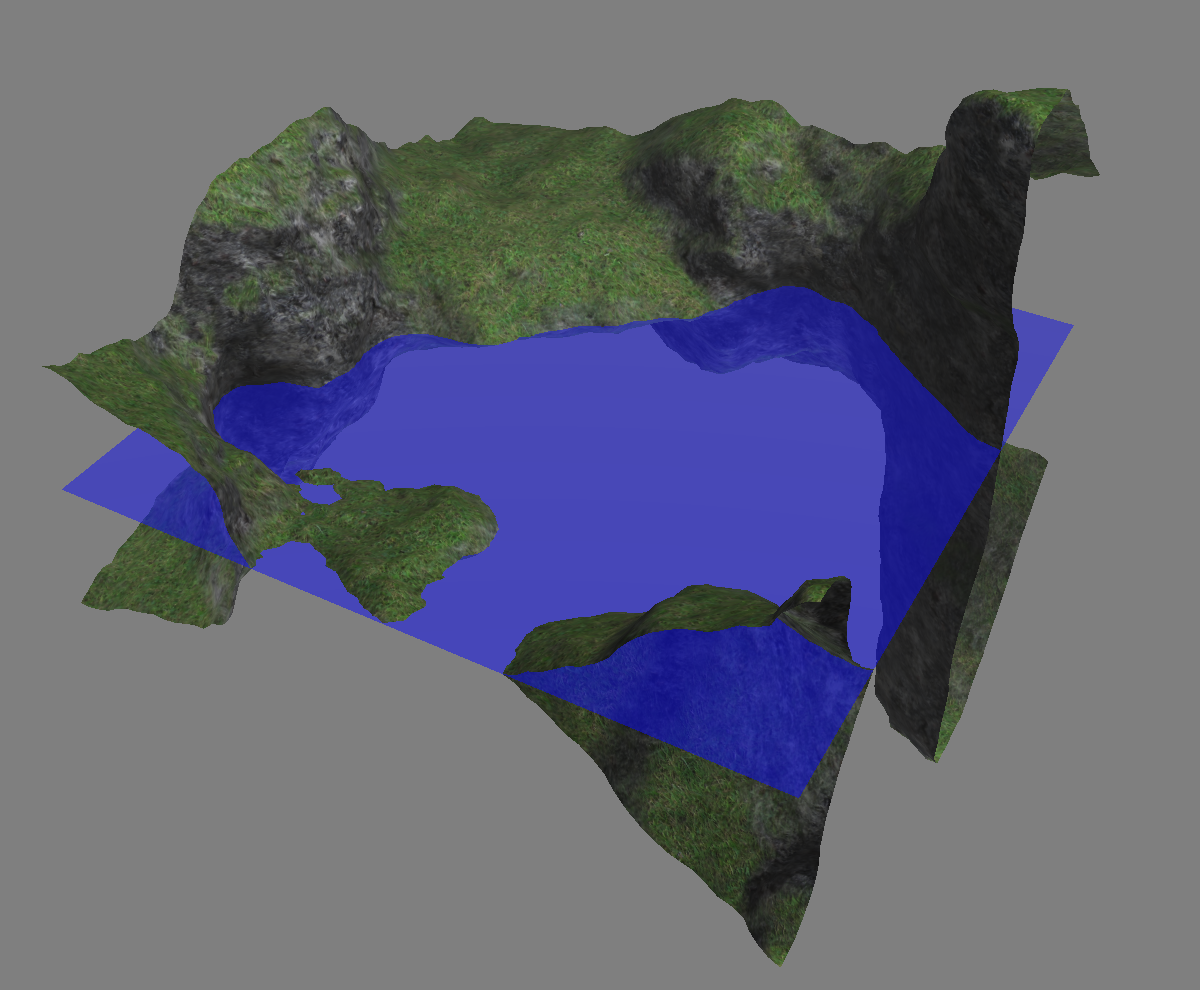
\includegraphics[width=8cm]{withoutstencil.png}
    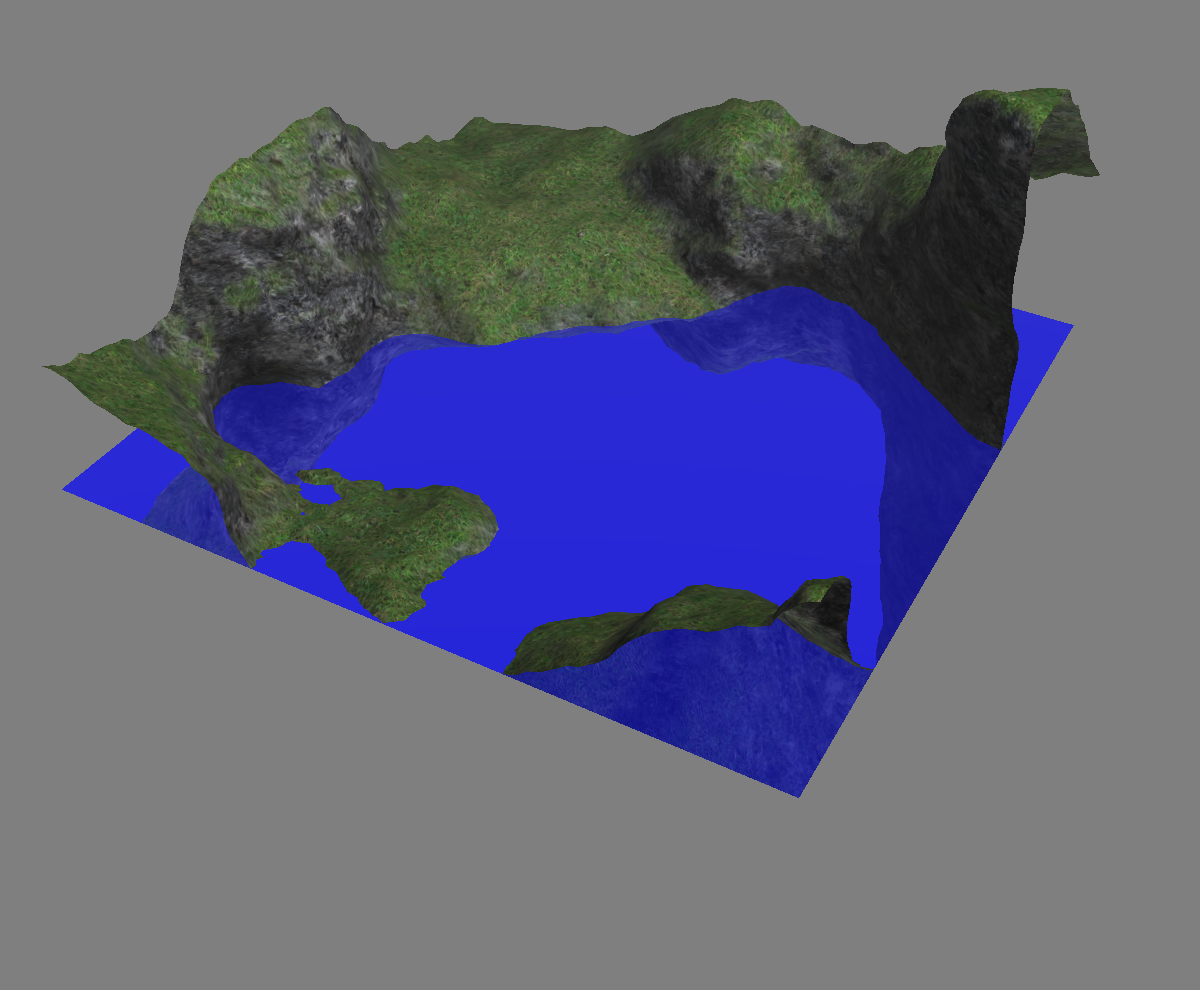
\includegraphics[width=8cm]{withstencil.png}
    without stencil (left), with stencil (right)
\end{center}

The advantage of this approach to rendering water is that it is simple. However, it is not very extensible. This implementation essentially uses water as a perfect mirror. In real life, it can be shown via ray optics that the properties of water behave differently depending on the viewing angle. If looking at water directly from above, it is possible to see through the water. However, if looking at water from the horizon, the water will tend to show reflection. Furthermore, it is difficult to simulate ripples using this technique. It may have been preferrable to render the water reflection to a texture instead, which would give more flexibility.

%----------------------------------------------------------------------------------------
\subsection{Level-of-Detail}

In order to show more geometry on the screen at once, we generate blocks far away at lower resolutions. More precisely, we generate blocks twice or four times as large, but with the same internal resolution (32x32x32). This is a better approach than generating blocks of the same size with a lower internal resolution since:

\begin{itemize}
\item We do not need to maintain three separate memory pools to store block vertices at different resolutions.
\item It is preferrable to avoid too many small allocations on the GPU.
\item Rendering more blocks is less efficient since it requires more CPU coordination (separate rendering commands need to be dispatched for each block, uniforms need to be changed, etc).
\end{itemize}

The size of the blocks can be visualized as such, where each block size is a different shade of gray. Note that some blocks overlap in the region where they transition from one to another.

\begin{center}
    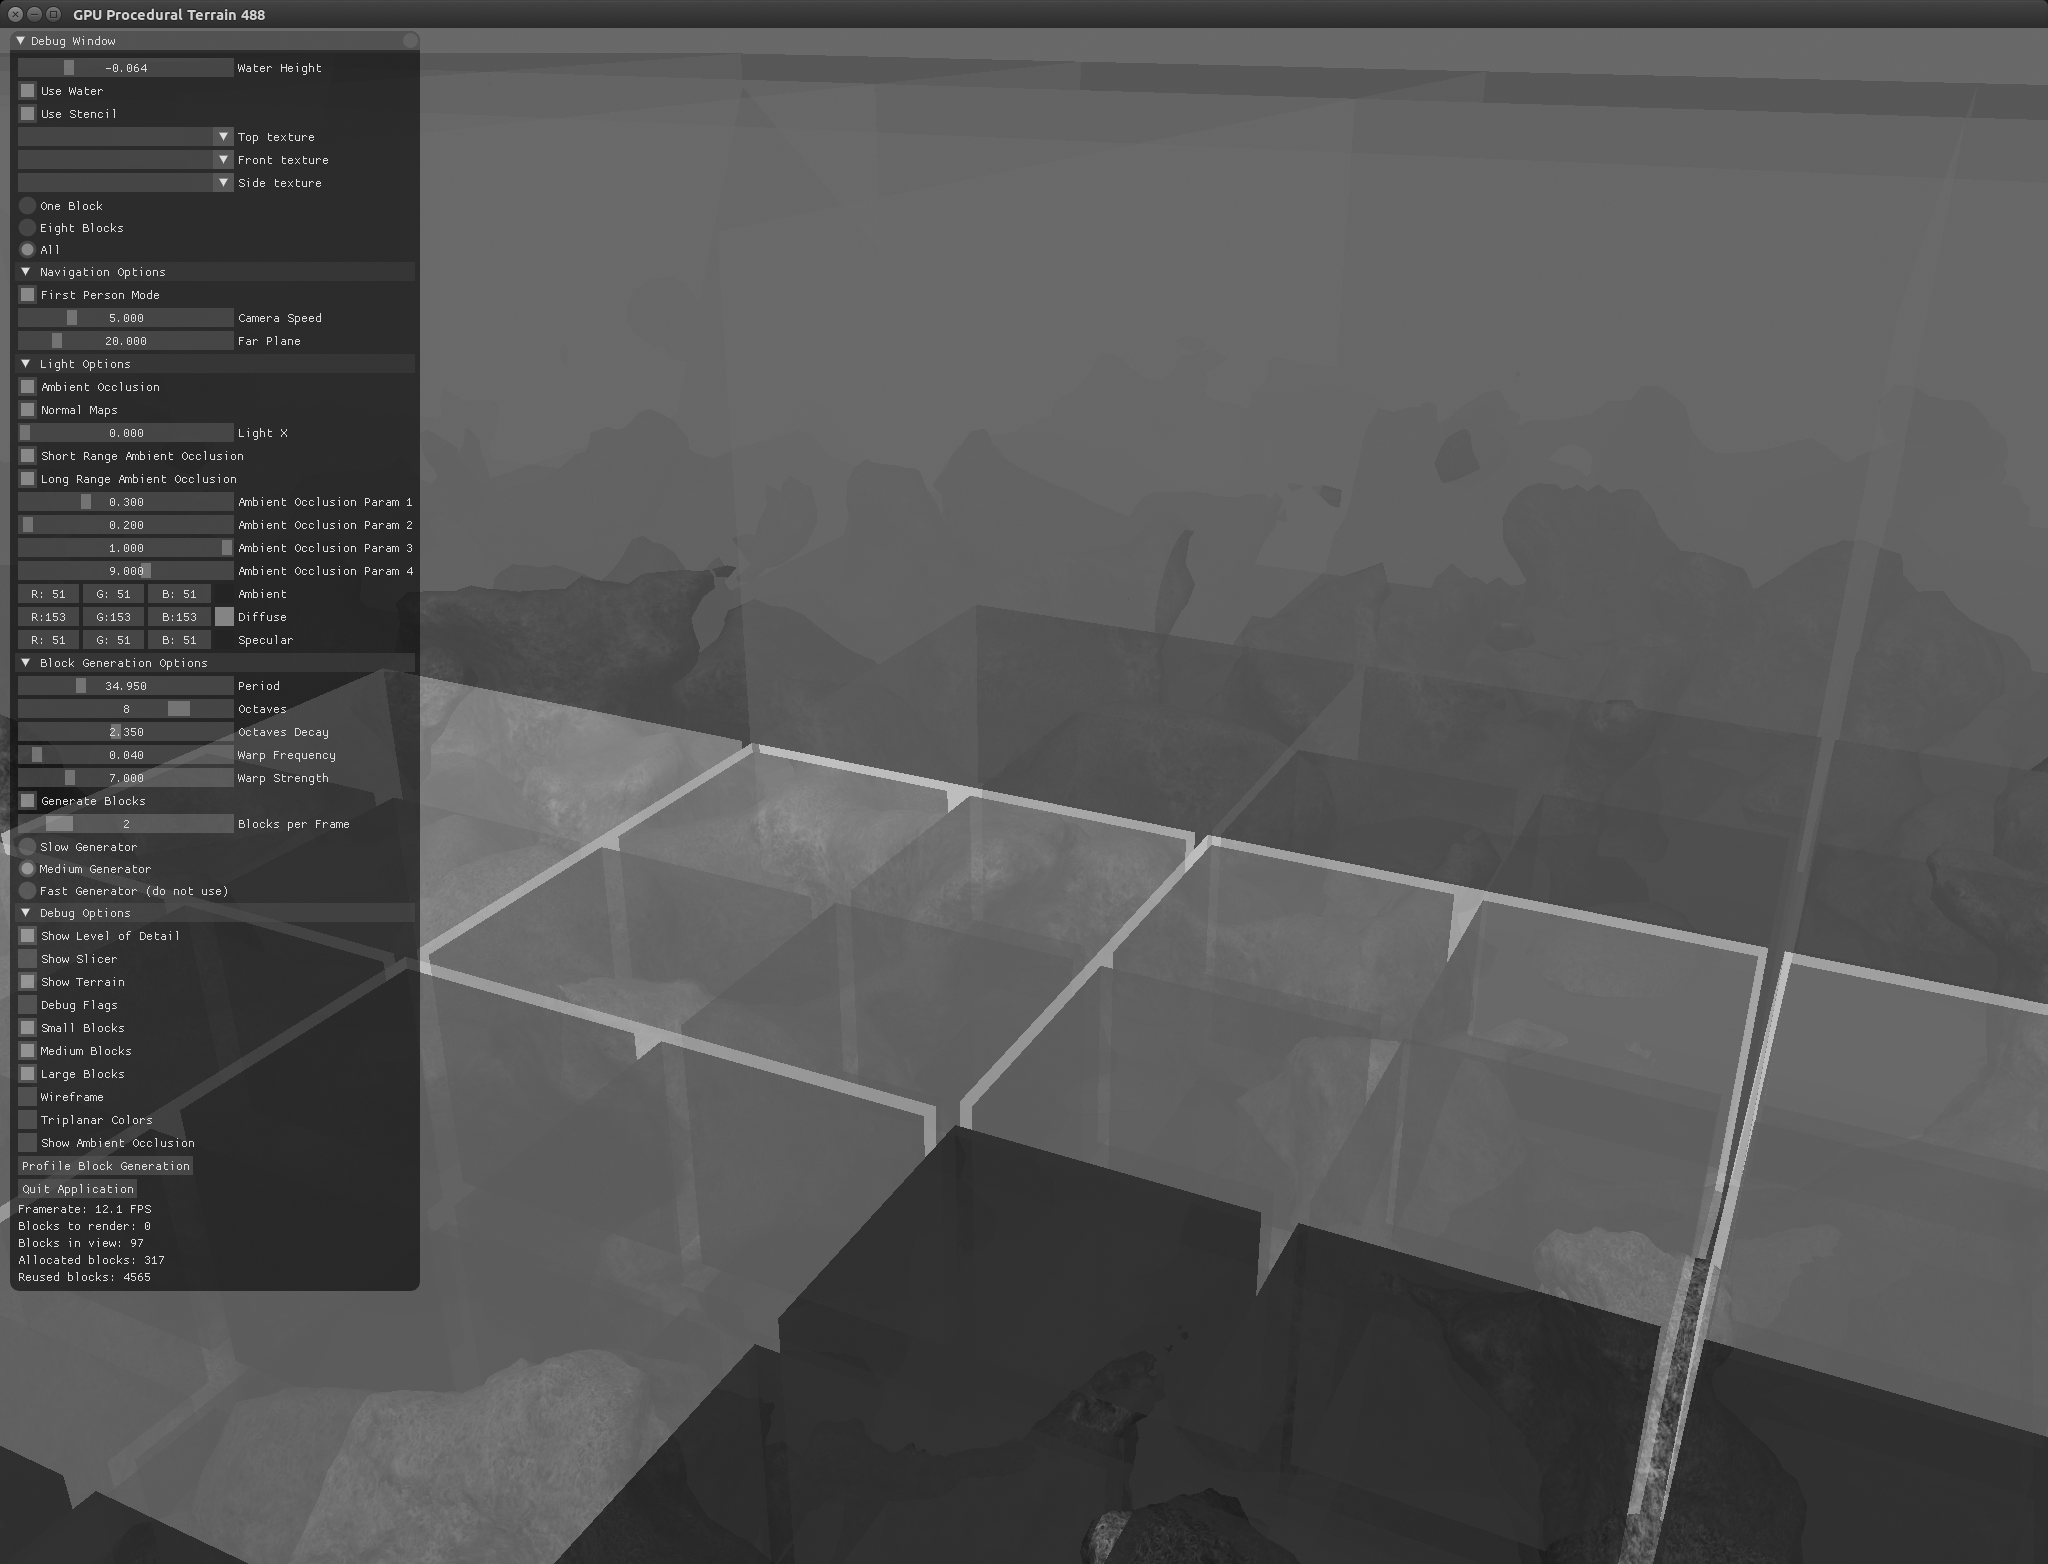
\includegraphics[width=12cm]{lod.png}

    level-of-detail visualization
\end{center}

In order to avoid sudden transitions, higher-resolution blocks fade-in as the camera moves closer to them. This can be done by adjusting the alpha component of the block's color. However, this technique only works if the high-resolution block is rendered in front of the medium-resolution block. To handle this problem, we ``erode'' the lower-resolution block by subtracting a small amount from the density function of the lower-resolution block. This handle the transition between blocks - however a side effect is that on occasions, the terrain ``grows'' as you approach it.

%----------------------------------------------------------------------------------------
%----------------------------------------------------------------------------------------
\section{Future Works}

There are many possible extensions to this project.

%----------------------------------------------------------------------------------------
\subsection{Robust Terrain Generation Engine}

This technique can be useful in randomized worlds, or as a mean of having complex terrain without to store a huge amount of data. However, to generate terrain interactively outside a demo, the requirements would be different. Areas to investigate include:

\begin{itemize}
\item Improve level-of-detail to make the transition between blocks of different resolutions even more seamless. It may be possible to come up with a smarter technique for `erosion' than simple subtracting from the density value.
\item Reduce the number of polygons rendered on the screen. As of now, storing terrain blocks on screen uses 2 GB of GPU memory, which is too much. This could be reduced with an adaptive marching cubes algorithm that uses a non-uniform polygon count for smooth/flat areas of the terrain. Additional techniques to simulate detail like displacement mapping \cite{Pharr:2005:GGP:1062395} can also help reduce polygon count.
\item Improve memory usage. Some data currently stored as floats could potentially be stored using half-floats or even chars.
\item Improve the performance of block generation. It is preferable to able to run this project without the latest GTX 980. Furthermore, in a demo, more than just the terrain would be rendered, meaning terrain generation alone should not take a significant percentage of computational time. The GPU Gems chapter presents a third technique for rendering block which is said to be 80\% faster, but it could not be implemented in time for the project deadline.
\item Render more terrain at distances further away, without relying on fog. The view range is not bad, but somewhat on the low side compared to open-world games.
\item Remove floating rocks by either 1) using the compute shader to perform a crude graph traversal or 2) sending rays from inside the geometry and measure the distance taken to exit the rock to see if it's likely a small floating rock.
\item Support character movement and collision detection.
\end{itemize}

%----------------------------------------------------------------------------------------
\subsection{Flexible Terrain Generation}

While the techniques presented in this report are sufficient for a visually pleasing demo, the user has minimal control over the shape of the terrain. In production, the artist may need to power to:

\begin{itemize}
\item Manually carve or extend the terrain by modifying the density value in certain areas. For example, by reducing the density values within an area defined by a cylinder, it would be possible to manually define a tunnel.
\item Have a better understanding of terrain generation parameters. Research needs to be done in finding more transformations to the density function to get different types of terrain shapes, and document them well to help the user achieve the desired configuration.
\item Add non-procedural geometry (e.g. a bridge, rocks) in a scene and adjust the surrounding terrain accordingly.
\item Control which texture gets used in which spot of the terrain (i.e. painting a texture).
\end{itemize}

%----------------------------------------------------------------------------------------
\subsection{Visual Effects}

\begin{itemize}
\item Volumetric light: it would be interesting to show sun rays \cite{Nguyen:2007:GG:1407436}\cite{GPUPro5}, also known as ``god rays''.
\item Hard shadows: while ambient occlusion is a nice approximation to soft shadows, there are cases where hard shadows are desirable, such as when a overhang or a large vertical structure is present.
\item Particle effects: As described in NVidia's ``Cascade'' demo \cite{Cascades}, it is possible to use particle effects to simulate a waterfall, running water, and ``wetness'' on the terrain.
\item Swarm effects: As described in NVidia's ``Cascade'' demo \cite{Cascades}, it is possible to add moving objects that learn to avoid the terrain by sampling the density function.
\item Vegetation: A grass texture is not sufficient to make a realistic landscape.
\item Better water: Implement water with refraction, ripples, animated textures, and a transition from refraction to reflection based on viewing angle.
\end{itemize}

%----------------------------------------------------------------------------------------
\subsection{Research}

The terrain generated using this technique are pleasing visually, but not necessarily realistic. Realism could be improved by attempting to simulate phenomenons such as:

\begin{itemize}
\item Erosion by air (often highly directional).
\item Erosion by water. This includes the generation of water pathways and sediment deposits.
\item Automatic terrain parameter configuration from real terrain data. It may be possible extract the properties of a real-terrain using, say, a 3D FFT, and find a way to add Perlin Noise at different frequencies and intensities (or some other kinds of random function) to approximate the frequency distribution.
\item Derive the right parameters in the program in a more systematic way. For example, the espilon used in calculating the normal from the gradient should probably vary as a function of terrain feature size.
\end{itemize}

Since we have a 3D density function, it may be interesting to modify this technique to render the terrain using distance-estimated ray-marching.

\bibliographystyle{plainurl}
\bibliography{sources}

\end{document}
